\section{Lecture 2: Lagrangian Mechanics, Euler-Lagrange Equation \& Hamiltonians}

\subsection{Lagrangian Mechanics \& Euler-Lagrange Equation}

Consider the following simplification: consider the case where the force $\mathbf{F}_\alpha$ is conservative. A force $\mathbf{F}_\alpha$ is \textbf{conservative} if:

\[
    \oint \mathbf{F}_\alpha \, d\mathbf{r}_\alpha = 0
\]

i.e., the work done to change the state of the system is independent of the path through the space of $\mathbf{r}_\alpha$. For a conservative force, 

\begin{align*}
    \mathbf{F}_\alpha &= \mathbf{\nabla}_\alpha V(\mathbf{r}_1,\ ...,\ \mathbf{r}_\alpha) \\
    &= - \frac{\partial}{\partial \mathbf{r}_\alpha} V(\mathbf{r}_1,\ ...,\ \mathbf{r}_\alpha)
\end{align*}

And the work done to change the state of the system from $\mathbf{r}_\alpha$ to $\mathbf{r}_\alpha^\prime$ is $V(\mathbf{r}_\alpha^\prime)-V(\mathbf{r}_\alpha)$. In this class, we will mostly consider conservative forces.

Since $\mathbf{r}_\alpha=\mathbf{r}_\alpha(q_i, t)$, we can write $V(\mathbf{r}_\alpha)$ as:

\[
    V(\mathbf{r}_\alpha)=V(q_i, t)
\]

From \textbf{Chain Rule}, we can get:

\[
    \frac{\partial V}{\partial q_i}=\sum_\alpha \frac{\partial V}{\partial \mathbf{r}_\alpha} \frac{\partial \mathbf{r}_\alpha}{\partial q_i}=-\sum_\alpha \mathbf{F}_\alpha \frac{\partial \mathbf{r}_\alpha}{\partial q_i}=-\mathbf{F}_i
\]

Then for a conservative force, we can get:

\[
    \frac{d}{dt} (\frac{\partial T}{\partial \dot{q}_i}) - \frac{\partial T}{\partial q_i} = -\frac{\partial V}{\partial q_i}
\]

Since $V$ is not a function of $q_i$, we can get:

\[
    \frac{\partial V}{\partial \dot{q}_i}=0
\]

So we can rewrite the EOM above by defining \textbf{Lagrangian} $L=T-V$, $L=L(q_i, \dot{q}_i, t)$

\[
    \frac{d}{dt} (\frac{\partial L}{\partial \dot{q}_i}) - \frac{\partial L}{\partial q_i} = 0
\]

This EOM is called \textbf{Euler-Lagrange Equation}. We can see that for a general dynamic system, if we can compute $L=T-V$, then we can find the equations of motion!

This is a set of $N$ differential equations, one for each DOF, where $N$ is the total number of DOF. Typically, these are $2^{\text{nd}}$ order ODEs for $q_i$.

To summarize, given a system of M parts and N degrees of freedom, it is advised to follow the following steps:

\begin{enumerate}
    \item Identify some dynamic variables $q_i$, and write down $\mathbf{r}_\alpha=\mathbf{r}_\alpha(q_i, t)$, where $\alpha=1,2,...,M$, $i=1,2,...,N$.
    \item Compute $T=\sum_\alpha \frac{1}{2} m_\alpha \dot{\mathbf{r}}_\alpha \cdot \dot{\mathbf{r}}_\alpha$ as a function of $q_i$.
    \item Compute $V=V(\mathbf{r}_\alpha)=V(q_i, t)$.
    \item Let $L=T-V$.
    \item We can get equations of motion: $\frac{d}{dt} (\frac{\partial L}{\partial \dot{q}_i}) - \frac{\partial L}{\partial q_i} = 0$.
\end{enumerate}

\begin{figure}[ht]
  \centering
  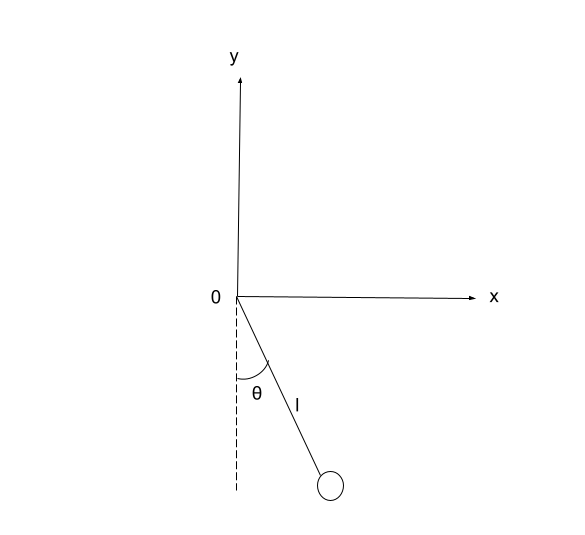
\includegraphics[width=0.8\textwidth]{images/2-1-1.png}
  \caption{Pendulum Example}
  \label{fig:2-1-1}
\end{figure}

For example, let's take a look at the pendulum in Figure \ref{fig:2-1-1}.

\begin{align*}
    x &= l \sin{\theta} \\
    y &= -l \cos{\theta} \\
\end{align*}

So we can get:

\begin{align*}
    \dot{x} &= l \cos{\theta} \cdot \dot{\theta} \\
    \dot{y} &= l \sin{\theta} \cdot \dot{\theta} \\
\end{align*}

So the kinetic energy can expressed as:

\[
    T=\frac{1}{2} m \left(\dot{x}^2+\dot{y}^2\right) = \frac{1}{2} ml^2\dot{\theta}^2
\]

The potential energy is:

\[
    V=-mgy=-mgl\cos{\theta}
\]

\[
    L=\frac{1}{2}ml^2\dot{\theta}^2+mgl\cos{\theta}
\]

From \textbf{Euler-Lagrange Equation} we can get:

\[
    ml^2\Ddot{\theta}+mgl\sin{\theta}=0
\]

This is exactly the same as we get using Newton's Law!

\subsection{Hamiltonian Mechanics}

The Lagrangian Mechanics is conceptually useful. But what if we step further? We have dynamic variables $q_i$, $L(q, q_i, t)$, so we define the \textbf{Hamiltonian} as $H=\sum_i \dot{q_i} \frac{\partial L}{\partial \dot{q_i}} - L$.

\[
    \frac{dH}{dt}=\sum_i \left(\Ddot{q_i} \frac{\partial L}{\partial \dot{q_i}} + \dot{q_i} \frac{d}{dt} \left(\frac{\partial L}{\partial \dot{q_i}}\right)\right) - \sum_i \left(\frac{\partial L}{\partial q_i} \dot{q_i} + \frac{\partial L}{\partial \dot{q_i}} \Ddot{q_i} \right) - \frac{\partial q_i}{\partial t}
\]

We know:

\[
    \frac{\partial L}{\partial q_i}=\frac{d}{dt} \left(\frac{\partial L}{\partial \dot{q_i}}\right)
\]

So we can get the following equation:

\[
    \frac{dH}{dt}=-\frac{\partial L}{\partial t}
\]

The total time derivative of $H$ is the explicit time derivative of $L$! If $L$ has no explicit time dependence, then we can get:

\[
    \frac{dH}{dt}=0
\]

i.e., $H$ is conserved.

So what is the \textbf{Hamiltonian}? If the constraints are time independent,

\[
    \mathbf{r}_\alpha=\mathbf{r}_\alpha (q_i)
\]

Then we can get

\[
    T=\frac{1}{2} \sum_\alpha m_\alpha \dot{\mathbf{r}_\alpha} \cdot \dot{\mathbf{r}_\alpha}
\]

\[
    \frac{\partial L}{\partial \dot{q_i}} = \frac{\partial T}{\partial \dot{q_i}} = \sum_\alpha m_\alpha \dot{\mathbf{r}}_\alpha \cdot \frac{\partial \dot{\mathbf{r}}_\alpha}{\partial \dot{q_i}} = \sum_\alpha m_\alpha \dot{\mathbf{r}}_\alpha \cdot \frac{\partial \mathbf{r}_\alpha}{\partial q_i}
\]

\begin{align*}
    \sum_i \dot{q_i} \frac{\partial L}{\partial q_i} &= \sum_i \dot{q_i} \left(\sum_\alpha m_\alpha \dot{\mathbf{r}}_\alpha  \frac{\partial \mathbf{r}_\alpha}{\partial q_i}\right) \\
    &= \sum_\alpha m_\alpha \dot{\mathbf{r}}_\alpha \left(\sum_i \frac{\partial r_\alpha}{\partial q_i} \dot{q_i}\right) \\
    &= \sum_\alpha m_\alpha \dot{\mathbf{r}}_\alpha \cdot \dot{\mathbf{r}}_\alpha \\
    &= 2T
\end{align*}

So we can get:

\begin{align*}
    H &= \sum_i \dot{q_i} \frac{\partial L}{\partial q_i} - L \\
    &= 2T - \left(T - V\right) \\
    &= T + V \\
\end{align*}

So $H$ is the total energy of the system (in many cases)!

We can get the following conclusions from the analysis above:

\begin{enumerate}
    \item If the \textbf{Lagrangian} $L$ is time independent, then the total energy of the system is conserved.
    \item If the \textbf{Lagrangian} $L$ is time independent, the system has time translation symmetry.
\end{enumerate}

So conserved energy is equivalent to time translation symmetry.

\begin{definition}[Noether's theorem]
    Every continuous symmetry of the action of a physical system with conservative forces has a corresponding conservation law.
\end{definition}

Let's look at another example of \textbf{Noether's theorem}: Imagine $L(q_i, \dot{q_i}, t)$ is 
independent of $q_i$ (although it could depend on $q_i$). In this way, we can represent 
$L=L(\dot{q_i}, t)$, so we can get:

\[
    \frac{d}{dt} \left(\frac{\partial L}{\partial \dot{q_i}}\right) = 0
\]

So $\frac{\partial L}{\partial \dot{q_i}}$ is conserved. This is the \textbf{momentum}!

\begin{definition}[Momentum]
    The \textbf{momentum} $p_i$ conjugated to $q_i$ is defined as $\frac{\partial L}{\partial \dot{q_i}}$.
    This momentum is conserved if the Lagrangian $L$ is independent of the coordinate $q_i$.
\end{definition}

At last, let's take a look at a particle moving in a circle. We have the following equations of motion:

\begin{align*}
    x&=R\cos(\theta)\\
    y&=R\sin(\theta)\\
\end{align*}

So we can get:

\begin{align*}
    \dot{x}&=-R\sin(\theta)\dot{\theta}\\
    \dot{y}&=R\cos(\theta)\dot{\theta}\\
\end{align*}

\[
    L = T = \frac{1}{2} m (\dot{x}^2+\dot{y}^2) = \frac{1}{2} m R^2 \dot{\theta}^2
\]

$L$ is independent of $\theta$.

\[
    p_\theta =  m R^2 \dot{\theta} = \text{angular momentum}
\]

In summary, a linear translation symmetry leads to conservation of momentum, a 
rotational symmetry leads to conservation of angular momentum, a time translation
symmetry leads to conservation of energy.